\documentclass{jsarticle}

\usepackage[dvipdfmx]{graphicx}
\usepackage{tikz}

\begin{document}

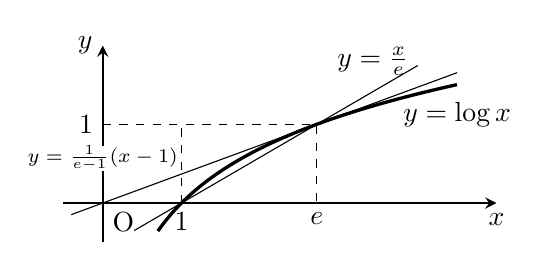
\begin{tikzpicture}

   % 座標軸
   \draw [thick, -stealth](-0.5,0)--(5,0) node [anchor=north]{$x$};
   \draw [thick, -stealth](0,-0.5)--(0,2) node [anchor=east]{$y$};
   \node [anchor=north west] at (0,0) {O};

   % y=log(x)
   \draw [very thick, domain=0.7:4.5, samples=200] plot(\x, {ln(\x)});
   \node [anchor=north] at (4.5,1.4){$y=\log x$};

   % y=x/e
   \draw [domain=-0.4:4.5] plot(\x,\x/e);
   \node [anchor=east] at(4,1.8){$y=\frac{x}{e}$};

   % y=(x-1)/(e-1)
   \draw [domain=0.4:4] plot(\x, {(\x-1)/(e-1)});
   \node [anchor=south, font=\scriptsize, fill=white, inner sep=0pt] at(0,0.4){$y=\frac{1}{e-1}(x-1)$};

   % 補助線
   \draw [dashed](0,1) node [anchor=east]{$1$}--(e,1)--(e,0) node[anchor=north]{$e$};
   \draw [dashed](1,0) node [anchor=north]{$1$}--(1,1);

\end{tikzpicture}

\end{document}